% ------------------------------------------------------------------ %
% Examination of a Bayesian approach to inverse kinematics.
% Andrew J. Pohl, Matthew R. Schofield & Reed Ferber
% Submitted to Journal of Biomechanics March 2021
% SupplementaryMaterialB.tex
% ------------------------------------------------------------------ %
\documentclass{article}
 \usepackage{setspace}

% ------------------------------------------------------------------ %
% Examination of a Bayesian approach to inverse kinematics.
% Andrew J. Pohl, Matthew R. Schofield & Reed Ferber
% Submitted to Journal of Biomechanics March 2021
% SupplementaryMaterial Structure
% structure.tex
% ------------------------------------------------------------------ %
%% Package inclusion
\usepackage[running]{lineno} % Line Numbers


 \usepackage[authoryear]{natbib}
\bibliographystyle{model5-names}

% SI 
\usepackage{siunitx}
% Hyper refferences
\usepackage{hyperref}

% Packages for tables
\usepackage{multirow}

% Packages for figures
\usepackage{subcaption}	

% Math Packages
\usepackage{amsmath,amsfonts,stmaryrd,amssymb, bm} 
\DeclareMathOperator*{\argmin}{argmin} 

\usepackage{enumerate} % Custom item numbers for enumerations

\usepackage[ruled]{algorithm2e} % Algorithms

\usepackage[framemethod=tikz]{mdframed} % Allows defining custom boxed/framed environments

\usepackage{listings} % File listings, with syntax highlighting
\lstset{
	basicstyle=\ttfamily, % Typeset listings in monospace font
}

%----------------------------------------------------------------
%	DOCUMENT MARGINS
%----------------------------------------------------------------

\usepackage{geometry} % Required for adjusting page dimensions and margins

\geometry{
	paper=letterpaper, % Paper size, change to letterpaper for US letter size
	top=2.5cm, % Top margin
	bottom=3cm, % Bottom margin
	left=2.5cm, % Left margin
	right=2.5cm, % Right margin
	headheight=14pt, % Header height
	footskip=1.5cm, % Space from the bottom margin to the baseline of the footer
	headsep=1.2cm, % Space from the top margin to the baseline of the header
	%showframe, % Uncomment to show how the type block is set on the page
}

%-------------------------------------------------------------------------
%	FONTS
%-------------------------------------------------------------------------

\usepackage[utf8]{inputenc} % Required for inputting international characters
\usepackage[T1]{fontenc} % Output font encoding for international characters

\usepackage{XCharter} % Use the XCharter fonts

%---------------------------------------------------------------------------
%	EMPHASISE ENVIRONMENT
%---------------------------------------------------------------------------

% Usage:
% \begin{emphasise}
%	\begin{verbatim}
%		$ ls
%		
%		Applications	Desktop	...
%	\end{verbatim}
% \end{commandline}

\mdfdefinestyle{emphasise}{
	leftmargin=10pt,
	rightmargin=10pt,
	innerleftmargin=15pt,
	middlelinecolor=black!50!white,
	middlelinewidth=2pt,
	frametitlerule=false,
	backgroundcolor=black!5!white,
	frametitle={Command Line},
	frametitlefont={\normalfont\sffamily\color{white}\hspace{-1em}},
	frametitlebackgroundcolor=black!50!white,
	nobreak,
}

% Define a custom environment for command-line snapshots
\newenvironment{emphasise}{
	\medskip
	\begin{mdframed}[style=emphasise]
}{
	\end{mdframed}
	\medskip
}

%--------------------------------------------------------------------------
%	FILE CONTENTS ENVIRONMENT
%--------------------------------------------------------------------------

% Usage:
% \begin{file}[optional filename, defaults to "File"]
%	File contents, for example, with a listings environment
% \end{file}

\mdfdefinestyle{file}{
	innertopmargin=1.6\baselineskip,
	innerbottommargin=0.8\baselineskip,
	topline=false, bottomline=false,
	leftline=false, rightline=false,
	leftmargin=2cm,
	rightmargin=2cm,
	singleextra={%
		\draw[fill=black!10!white](P)++(0,-1.2em)rectangle(P-|O);
		\node[anchor=north west]
		at(P-|O){\ttfamily\mdfilename};
		%
		\def\l{3em}
		\draw(O-|P)++(-\l,0)--++(\l,\l)--(P)--(P-|O)--(O)--cycle;
		\draw(O-|P)++(-\l,0)--++(0,\l)--++(\l,0);
	},
	nobreak,
}

% Define a custom environment for file contents
\newenvironment{file}[1][File]{ % Set the default filename to "File"
	\medskip
	\newcommand{\mdfilename}{#1}
	\begin{mdframed}[style=file]
}{
	\end{mdframed}
	\medskip
}

%--------------------------------------------------------------------------
%	NUMBERED QUESTIONS ENVIRONMENT
%--------------------------------------------------------------------------

% Usage:
% \begin{question}[optional title]
%	Question contents
% \end{question}

\mdfdefinestyle{question}{
	innertopmargin=1.2\baselineskip,
	innerbottommargin=0.8\baselineskip,
	roundcorner=5pt,
	nobreak,
	singleextra={%
		\draw(P-|O)node[xshift=1em,anchor=west,fill=white,draw,rounded corners=5pt]{%
		Question \theQuestion\questionTitle};
	},
}

\newcounter{Question} % Stores the current question number that gets iterated with each new question

% Define a custom environment for numbered questions
\newenvironment{question}[1][\unskip]{
	\bigskip
	\stepcounter{Question}
	\newcommand{\questionTitle}{~#1}
	\begin{mdframed}[style=question]
}{
	\end{mdframed}
	\medskip
}

%-------------------------------------------------------------------------
%	WARNING TEXT ENVIRONMENT
%-------------------------------------------------------------------------

% Usage:
% \begin{warn}[optional title, defaults to "Warning:"]
%	Contents
% \end{warn}

\mdfdefinestyle{warning}{
	topline=false, bottomline=false,
	leftline=false, rightline=false,
	nobreak,
	singleextra={%
		\draw(P-|O)++(-0.5em,0)node(tmp1){};
		\draw(P-|O)++(0.5em,0)node(tmp2){};
		\fill[black,rotate around={45:(P-|O)}](tmp1)rectangle(tmp2);
		\node at(P-|O){\color{white}\scriptsize\bf !};
		\draw[very thick](P-|O)++(0,-1em)--(O);%--(O-|P);
	}
}

% Define a custom environment for warning text
\newenvironment{warn}[1][Warning:]{ % Set the default warning to "Warning:"
	\medskip
	\begin{mdframed}[style=warning]
		\noindent{\textbf{#1}}
}{
	\end{mdframed}
}

%------------------------------------------------------------------------
%	INFORMATION ENVIRONMENT
%------------------------------------------------------------------------

% Usage:
% \begin{info}[optional title, defaults to "Info:"]
% 	contents
% 	\end{info}

\mdfdefinestyle{info}{%
	topline=false, bottomline=false,
	leftline=false, rightline=false,
	nobreak,
	singleextra={%
		\fill[black](P-|O)circle[radius=0.4em];
		\node at(P-|O){\color{white}\scriptsize\bf i};
		\draw[very thick](P-|O)++(0,-0.8em)--(O);%--(O-|P);
	}
}

% Define a custom environment for information
\newenvironment{info}[1][Info:]{ % Set the default title to "Info:"
	\medskip
	\begin{mdframed}[style=info]
		\noindent{\textbf{#1}}
}{
	\end{mdframed}
}
 % Include the file specifying the document structure and custom commands

\renewcommand{\thefigure}{B\arabic{figure}}
\setcounter{figure}{0}

\renewcommand{\thetable}{B\arabic{table}}
\setcounter{table}{0}

%--------------------------------------------------------------------%

\title{Supplementary Material B - Random Initial Values} % Title of the assignment

\author{Andrew J. Pohl, Matthew R. Schofield \&  Reed Ferber} % Author name and email address

\date{University of Calgary \today} % University, school and/or department name(s) and a date

%-----------------------------------------------------------------------%

\begin{document}
\linenumbers
\maketitle % Print the title
\doublespacing

Both numerical optimisation used for least squares (LS) methods and MCMC used for Bayesian inference require the specification of initial values, the choice of which can influence the output of each respective algorithm.  Unlike the main article in which the true values of each simulation were used as initial values for numerical minimisation of LS error and the resulting LS estimate used to initialise MCMC sampling, this appendix focus on the performance of each model when initial values are specified randomly. For LS optimisation this equates to selecting initial values with uniform probability from the support of each parameter. For MCMC sampling this equates to selecting initial values at random from the prior distribution for the respective Bayesian model.  All research code to replicate this analysis can be found at: \href{https://github.com/AndyPohlNZ/BayesKin}{https://github.com/AndyPohlNZ/BayesKin}.

\section{Results}
Performance of each model on identifying underling pose parameters when random values are used as initial values for MCMC sampling or numerical optimisation are presented for 1, 2 and 3-link chains in Figures \ref{fig:StripChart_SingleLink_Random}, \ref{fig:StripChart_DoubleLink_Random}, \ref{fig:StripChart_random} respectfully and the bias, variance and RMSE for each model are presented in Table \ref{tab:BiasVarianceRMSE_random} Distinctive banding at non-optimal estimators occurs in all models with the exception of the third set of priors for the Bayesian model.  This is reflected in increased bias, variance, and RMSE for P1, P2 and LS models.

\begin{figure}
\centering
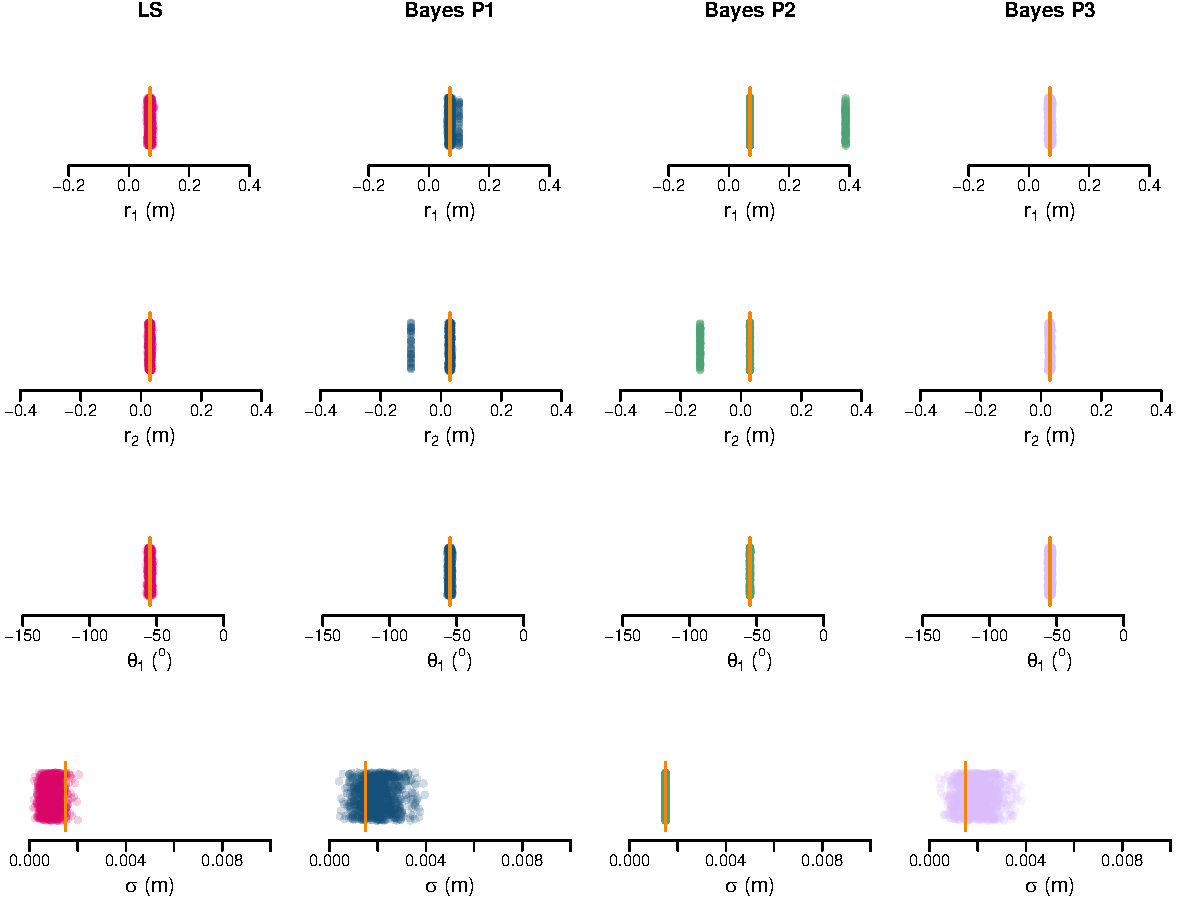
\includegraphics[width=\textwidth]{./Figures/SingleLink_StripChart_random.pdf}
\caption{Performance of the estimators from each model (columns) on each parameter (rows) for 1000 single link simulations where initial values were specified using random values.  True values for each parameter identified in orange.}
\label{fig:StripChart_SingleLink_Random}
\end{figure}

\begin{figure}
\centering
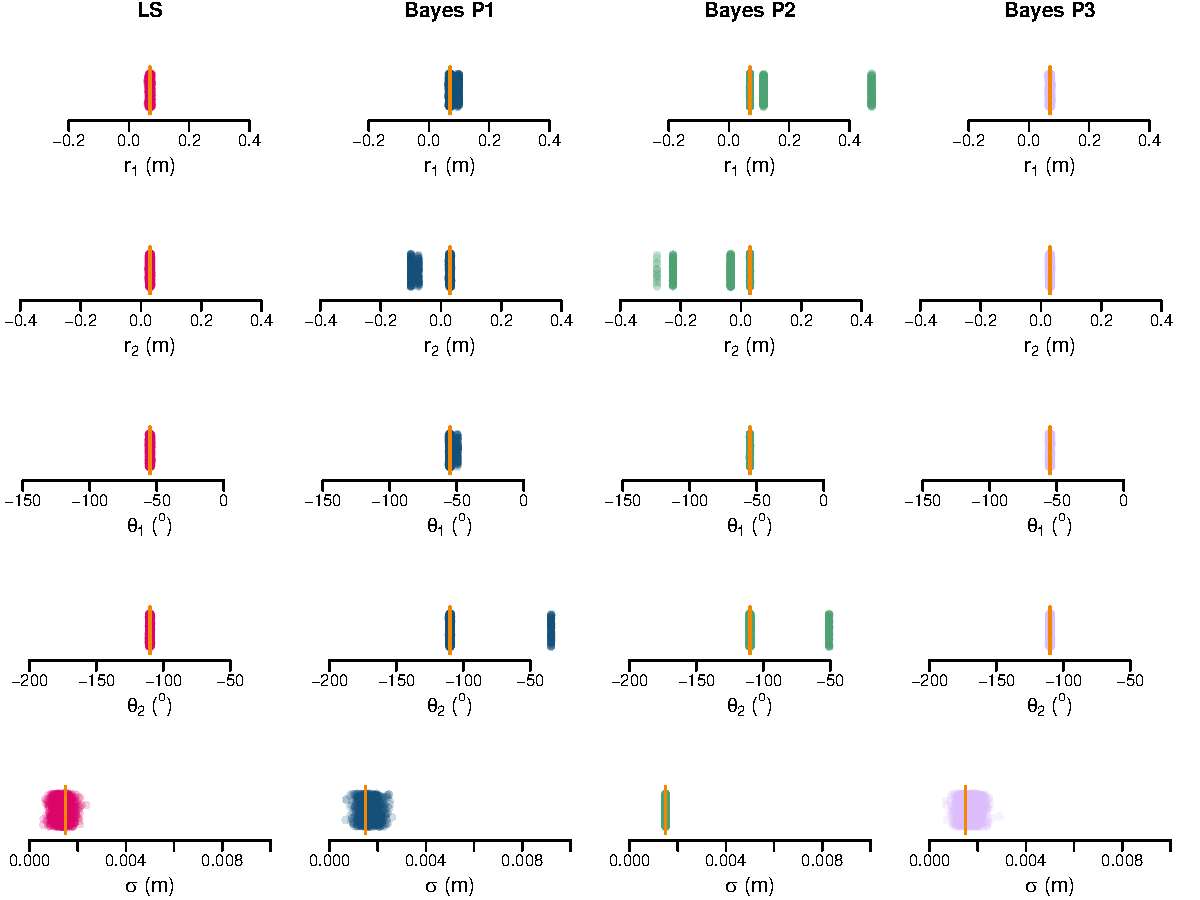
\includegraphics[width=\textwidth]{./Figures/DoubleLink_StripChart_random.pdf}
\caption{Performance of the estimators from each model (columns) on each parameter (rows) for 1000 double link simulations where initial values were specified using random values.  True values for each parameter identified in orange.}
\label{fig:StripChart_DoubleLink_Random}
\end{figure}

\begin{figure}
\centering
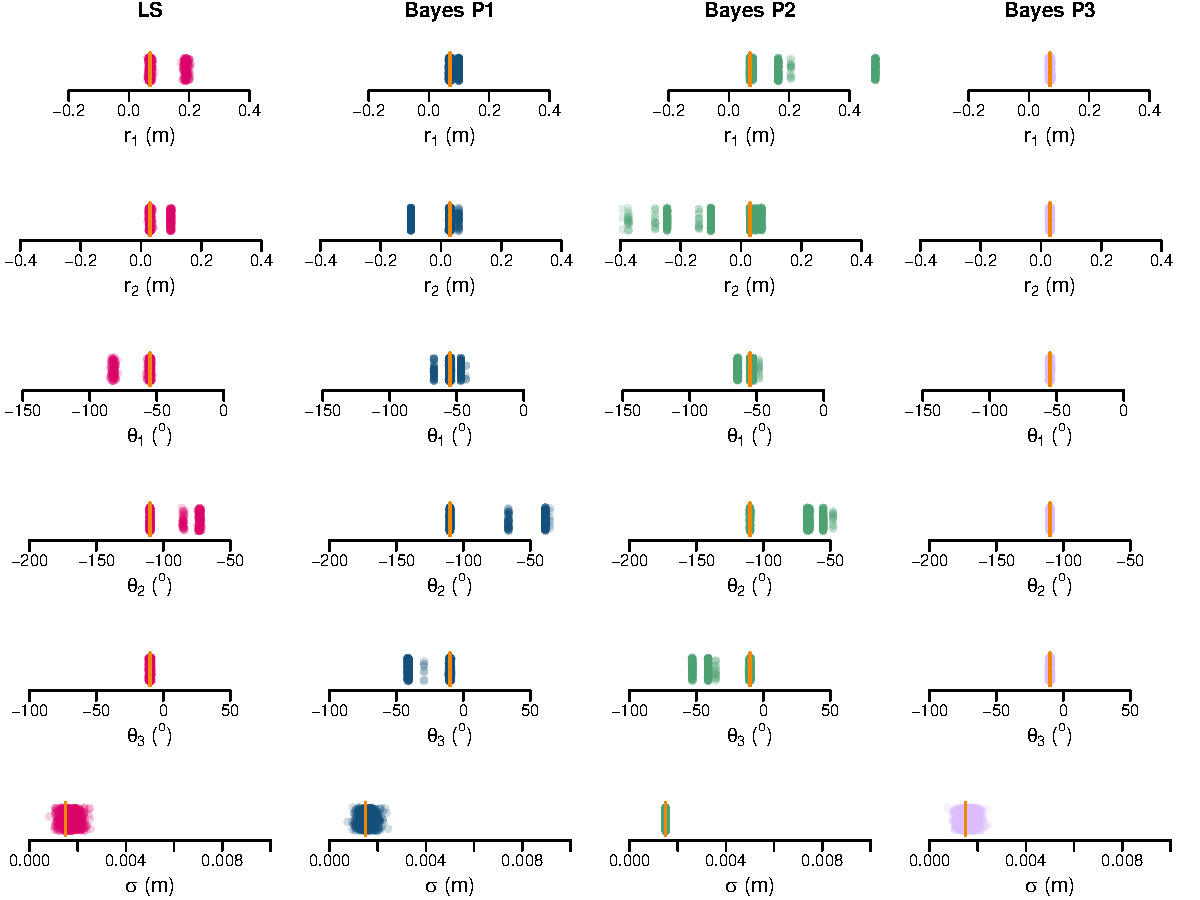
\includegraphics[width=\textwidth]{./Figures/TripleLink_StripChart_random.pdf}
\caption{Performance of the estimators from each model (columns) on each parameter (rows) 1000 triple link simulations where initial values were specified using random values.  True values for each parameter identified in orange.}
\label{fig:StripChart_random}
\end{figure}



\begin{table}
\centering
\resizebox{\textwidth}{!}{%
\begin{tabular}{ll cccc cccc cccc cccc}
  \hline
  && & \multicolumn{3}{c}{LS} && \multicolumn{3}{c}{Bayes P1} && \multicolumn{3}{c}{Bayes P2} && \multicolumn{3}{c}{Bayes P3}\\
  && & Bias & Variance & RMSE && Bias & Variance & RMSE && Bias & Variance & RMSE && Bias & Variance & RMSE\\
  \hline
  \multirow{4}{*}{Single Link}  && $r_1 \, (\si{\milli\meter})$ & $-0.029$ & $18.459$ & $4.297$ &&
                                    $1.556$ & $56.497$ & $7.676$ &&
                                    $44.100$ & $12058.962$ & $118.337$ &&
                                    $-0.260$ & $13.221$ & $3.645$\\
                                && $r_2\, (\si{\milli\meter})$ & $-0.073$ & $9.486$ & $3.081$ &&
                                    $-6.855$ & $833.156$ & $29.667$ &&
                                    $-22.956$ & $3266.412$ & $61.591$ &&
                                    $-0.300$ & $6.788$ & $2.623$\\
                                && $\theta_1 \, (^{\circ})$ & $59.77$ & $0.847$ & $0.920$ &&
                                    $12.23$ & $0.603$ & $0.776$ &&
                                     $32.66$ & $0.020$ & $0.141$ &&
                                     $0.072$ & $0.608$ & $0.782$ \\
                                && $\sigma\, (\si{\milli\meter})$ & $-0.609$ & $0.092$ & $0.680$ &&
                                    $1.152$ & $8.751$ & $3.175$ &&
                                     $0.000$ & $<0.001$ & $<0.001$ &&
                                     $0.461$ & $0.375$ & $0.766$ \\
  \hline
  \multirow{5}{*}{Double Link}  && $r_1 \, (\si{\milli\meter})$ & $-0.045$ & $6.704$ & $2.590$ &&
                                    $5.322$ & $122.894$ & $12.297$ &&
                                    $68.903$ & $21234.964$ & $161.191$ &&
                                    $0.065$ & $5.330$ & $2.310$ \\
                                && $r_2\, (\si{\milli\meter})$ & $0.005$ & $4.653$ & $2.157$ &&
                                    $-22.887$ & $2234.145$ & $52.516$ &&
                                    $-50.044$ & $8325.410$ & $104.067$ &&
                                    $0.094$ & $3.561$ & $1.889$\\
                                && $\theta_1\, (^{\circ})$ & $ 79.20 $ & $0.272$ & $0.522$ &&
                                    $25.61$ & $0.202$ & $0.449$ &&
                                    $33.84$ & $0.010$ & $0.102$ &&
                                    $-0.020$ & $0.202$ & $0.451$\\
                                && $\theta_2\, (^{\circ})$ & $85.34$ & $0.170$ & $0.413$ &&
                                    $34.10$ & $0.127$ & $0.356$ &&
                                    $68.18$ & $0.087$ & $0.294$ &&
                                    $0.039$ & $0.127$ & $0.358$\\
                                && $\sigma\, (\si{\milli\meter})$ & $-0.158$ & $0.073$ & $0.314$ &&
                                    $2.721$ & $27.815$ & $5.935$ &&
                                    $0.000$ & $<0.001$ & $<0.001$ &&
                                    $0.150$ & $0.104$ & $0.355$\\
  \hline
  \multirow{6}{*}{Triple Link}  && $r_1\, (\si{\milli\meter})$ & $18.202$ & $1862.157$ & $46.834$ &&
                                    $8.275$ & $175.028$ & $15.605$ &&
                                    $93.421$ & $27338.532$ & $189.911$ &&
                                     $0.013$ & $4.976$ & $2.231$\\
                                && $r_2\, (\si{\milli\meter})$ & $10.584$ & $612.644$ & $26.920$ &&
                                    $-28.887$ & $3165.409$ & $63.244$ &&
                                     $-66.770$ & $13884.938$ & $135.437$ &&
                                     $0.071$ & $3.185$ & $1.786$ \\
                                && $\theta_1\, (^{\circ})$ & $75.99$ & $0.252$ & $0.502$ &&
                                    $32.83$ & $0.183$ & $0.428$ &&
                                    $35.22$ & $0.010$ & $0.098$ &&
                                    $-0.008$ & $0.183$ & $0.429$ \\
                                && $\theta_2\, (^{\circ})$ & $91.20$ & $0.052$ & $0.227$ &&
                                    $41.82$ & $0.038$ & $0.196$ &&
                                    $81.72$ & $0.026$ & $0.161$ &&
                                    $0.014$ & $0.039$ & $0.197$ \\
                                && $\theta_3\, (^{\circ})$ & $16.83$ & $0.229$ & $0.479$ &&
                                    $5.63$ & $0.166$ & $0.408$ &&
                                    $0.99$ & $0.146$ & $0.383$ &&
                                    $-0.046$ & $0.166$ & $0.408$ \\
                                && $\sigma\, (\si{\milli\meter})$ & $15.512$ & $966.393$ & $34.716$ &&
                                    $3.944$ & $37.030$ & $7.252$ &&
                                    $0.000$ & $<0.001$ & $<0.001$ &&
                                    $0.082$ & $0.065$ & $0.267$ \\
  \hline
\end{tabular}

}
\caption{Bias, Variance and RMSE of estimators for each model on single, double and triple link simulations when random values are used as initial conditions.  The equivalent results using random values for initial conditions can be found in table 1 in the main article.}
\label{tab:BiasVarianceRMSE_random}
\end{table}

\section{Discussion}
The banding of estimators highlighted in Figures \ref{fig:StripChart_SingleLink_Random} \ref{fig:StripChart_DoubleLink_Random} and \ref{fig:StripChart_random} suggests that there exists local minima within the LS cost surface or multimodality within the Bayesian Posterior.  This is supported by the partial cost surface highlighted Figure \ref{fig:LSCostFigs}.  We can see that the the numerical optimiser settles close to a small local minimum and that this local minima corresponds to a solution which matches marker plates located on the first two links despite having \ang{156} of error for $\theta_3$ and \SI{0.14}{\meter} of error for $\bm{r}$.  Such a solution could be described as a reflection of links 1 and 2 to approximately align the first two marker plates.  A similar phenomenon occurs when examining trace plots of MCMC chains for the same example (Figure \ref{fig:Traceplot_random}).  It is clear that poor mixing occurs between chains suggestive of a chain becoming `stuck' at this reflective solution and suggesting multimodality within the posterior.  

\begin{figure}
     \centering
     \begin{subfigure}[b]{0.45\textwidth}
         \centering
         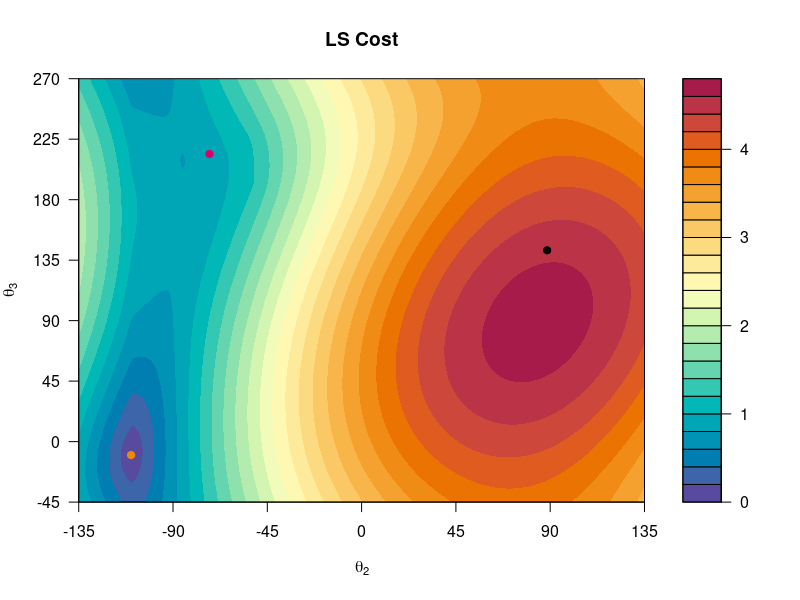
\includegraphics[width=\textwidth]{./Figures/LSCost.png}
         \caption{}
         \label{fig:LSCost}
     \end{subfigure}
     \hfill
     \begin{subfigure}[b]{0.45\textwidth}
         \centering
         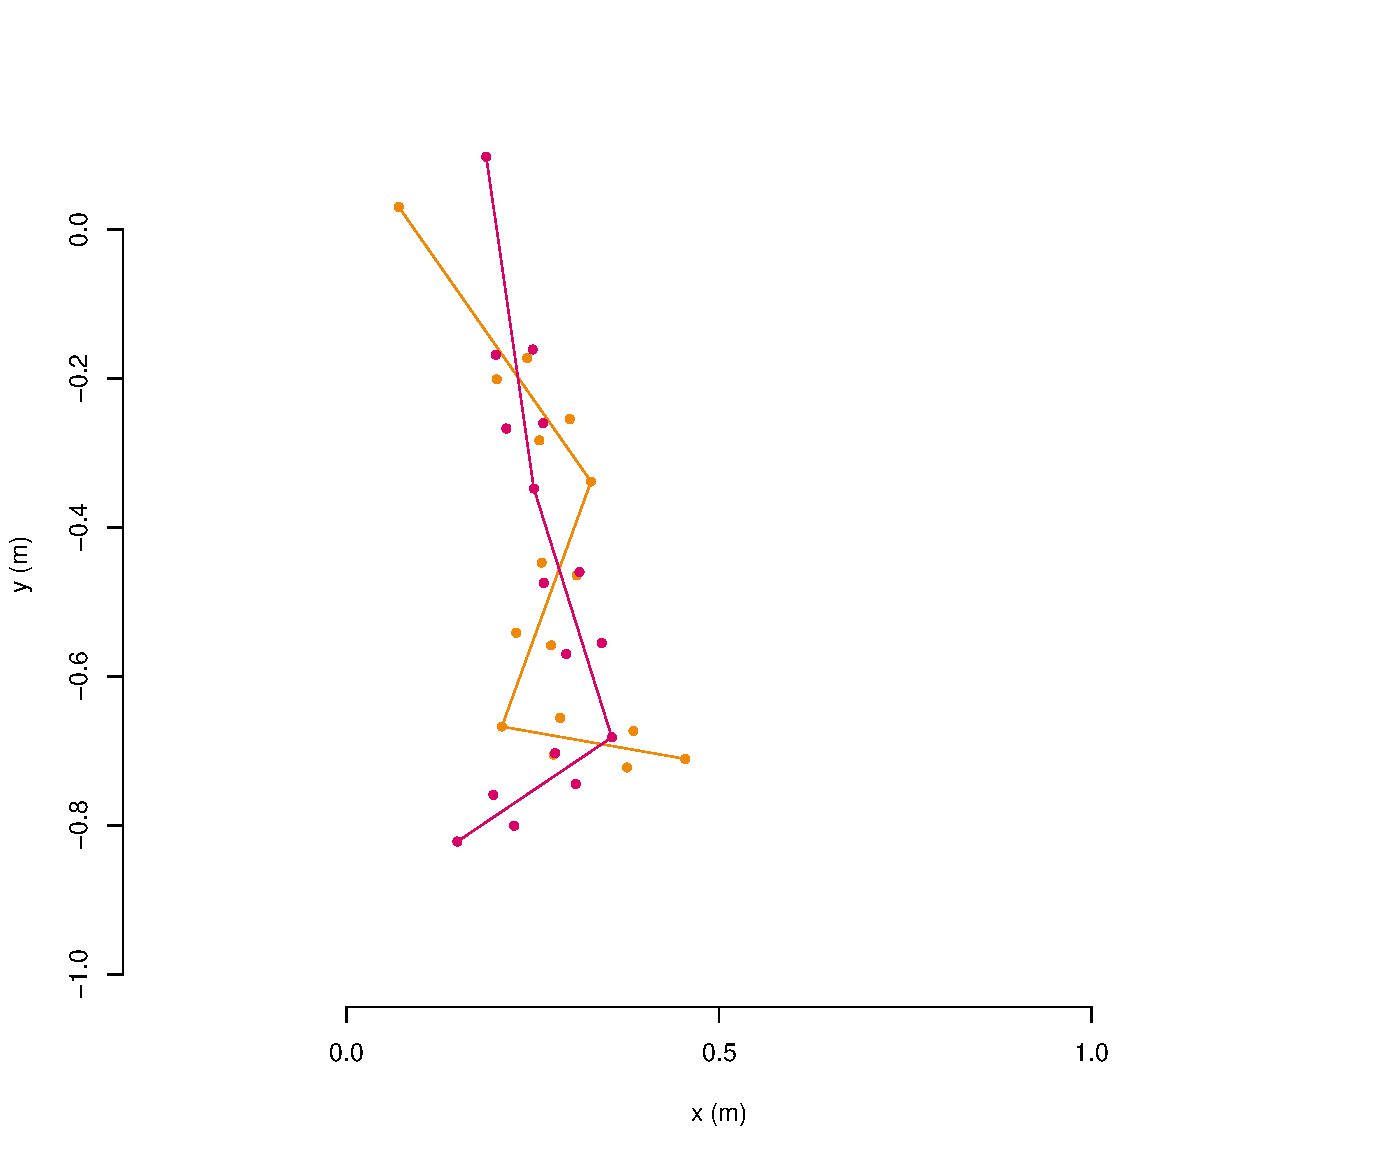
\includegraphics[width=\textwidth]{./Figures/LSCostPoses.pdf}
         \caption{}
         \label{fig:LSCostPose}
     \end{subfigure}
             \caption{Partial cost surface for a typical example of poor performance of the LS model on a 3-link problem \ref{fig:LSCost}.  In figure (a) the orange point denotes the true value, pink the result of optimisation and the black point the initial value.  In (b) the resulting pose estimate (pink) is compared to the true value (orange).}
        \label{fig:LSCostFigs}
\end{figure}


This is a well known problem both within the biomechanics community and in general the effect of initial values is well understood for optimisation problems.  Iterative methods such as the quasi-Newton BFGS method used in this work can settle on local optima or at saddle points where gradients change sign. Alternative optimisation algorithms such as simulated annealing \citep{bertsimas_simulated_1993}, may be effective at preventing numerical optimisation from settling on these local minima.

For MCMC based sampling in theory the specification of initial values does not prevent the samples from being obtained from the appropriate posterior distribution.  However, these theoretical arguments are made on the basis of asymptotic theory \citep{gilks_markov_1996}.  In practice we must terminate sampling at some finite value and as a result we hope that independent MCMC chains show adequate mixing to have confidence in the MCMC samples obtained. When random values were used to initiate MCMC chains we observe considerably higher $\hat{R}$ statistics \citep{brooks_general_1998} than when the true values were specified as a result $56\%$ of simulations were excluded on the basis of poor convergence (much higher than the $<0.1\%$ excluded when true values were specified).  

In Figure \ref{fig:Traceplot_random} a typical example of poor convergence is provided where independent Markov Chains become 'stuck' at different modes of the posterior distribution.  These modes correspond to the true solution and the `reflective' solution highlighted in \ref{fig:LSCostPose}.  In practice several solutions exist, in an analogous manner to simulated annealing for LS optimisation simulated tempering \citep{marinari_simulated_1992} provides a modification to MCMC sampling which improves sampling efficiency for multi-modal posteriors. Alternatively weakly informative priors (such as that proposed in Bayes P3) are not as effected by this phenomenon.  The `reflective' solution obtained in the case of random initial values pertains to a pose with extreme amount of ankle dorsiflexion or hip rotation, well beyond normal anatomical limits.  Such solutions have little prior probability if prior distributions are based on previous literature which describes the normal range of anatomically plausible motion as with our third set of priors.  A similar approach could be used for LS sampling in that the support of parameter values of which initial values are sampled from is limited to those based on previous literature.

\begin{figure}
\centering
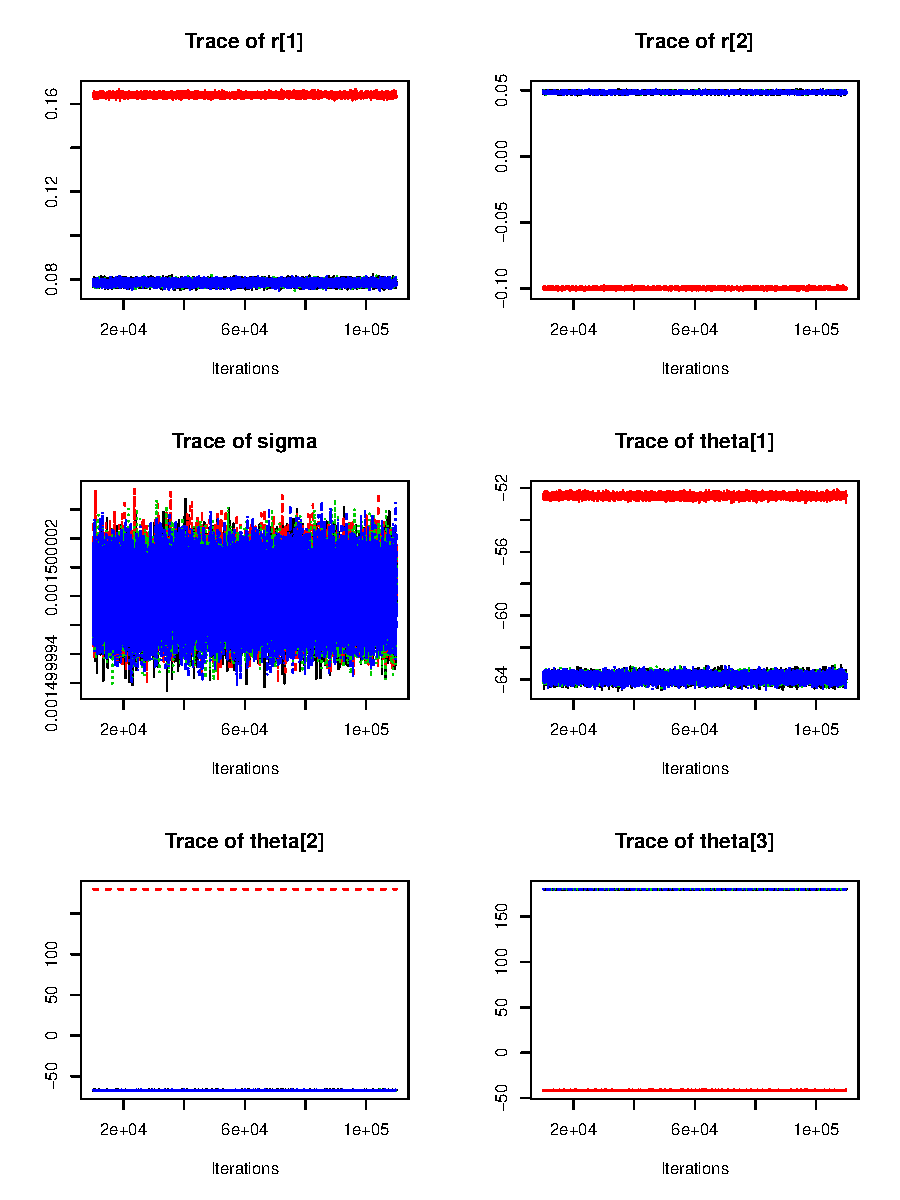
\includegraphics[width=\textwidth]{./Figures/traceplot_poor.pdf}
\caption{Traceplots demonstrating poor convergence with chains sampling from distinctively different modes within the posterior distribution.}
\label{fig:Traceplot_random}
\end{figure}

\bibliography{References.bib}


\end{document}}
